\documentclass{beamer}

\usetheme{CambridgeUS}

\usepackage{amsmath}
\usepackage{graphicx}
\usepackage{tfrupee}

% FOR TABLE (according to table generated by ssconvert)
\def\inputGnumericTable{}
\usepackage[latin1]{inputenc}
\usepackage{color}
\usepackage{array}
\usepackage{longtable}
\usepackage{calc}
\usepackage{multirow}
\usepackage{hhline}
\usepackage{ifthen}
\usepackage{lscape}

\providecommand{\pr}[1]{\ensuremath{\Pr\left(#1\right)}}

\title{Random Numbers}
\author{Kartheek Tammana}
\date{\today}
\logo{\large \LaTeX{}}

\begin{document}

\begin{frame}
    \titlepage
\end{frame}

\logo{}

\begin{frame}{Outline}
    \tableofcontents
\end{frame}

\section{Question 1}
\subsection{Question 1.1}
\begin{frame}{1.1 - Generating U}
    The random number generation is done in \texttt{./codes/gen\_uniform.c}.
\end{frame}

\subsection{Question 1.2}
\begin{frame}{1.2 - Graph of CDF of U}
    \begin{figure}[!ht]
        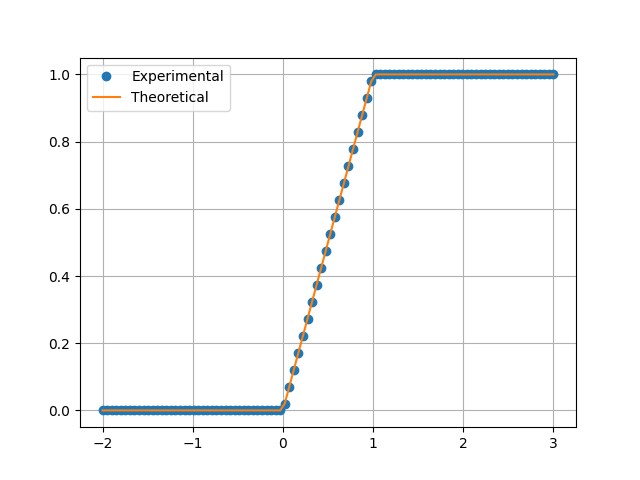
\includegraphics[width=\textheight]{figs/cdf_uni.png}
    \end{figure}
\end{frame}

\subsection{Question 1.3}
\begin{frame}{1.3 - CDF of U}
    The PDF of $U$ is given by
    \begin{equation}
        p_U(x) = 
        \begin{cases}
            1 & 0 \leq x \leq 1 \\
            0 & otherwise
        \end{cases} \label{eq:pu}
    \end{equation}
    And so we can find the CDF,
    \begin{align}
        F_U(x) &= \int_{-\infty}^{x}{p_U(x) dx} \\
        F_U(x) &=
        \begin{cases}
            0 & x < 0 \\
            x & 0 \leq x \leq 1 \\
            1 & x > 1
        \end{cases} \label{eq:fu}
    \end{align}
\end{frame}

\subsection{Question 1.4}
\begin{frame}{1.4 - Mean and variance of U}
    The mean and variance are calculated in \texttt{./codes/mean\_var.c}, if \texttt{./codes/uni.dat} is piped into \texttt{stdin}.
\end{frame}

\subsection{Question 1.5}
\begin{frame}{1.5 - Verification}
    We need to find
    \begin{equation}
        E\left[U^k\right] = \int_{-\infty}^{+\infty}{x^k d F_U(x)}
    \end{equation}

    But
    \begin{equation}
        d F_U(x) = p_U(x) dx
    \end{equation}

    So from eq \eqref{eq:pu}, we have
    \begin{align}
        E\left[U^k\right] &= \int_{-\infty}^{+\infty}{x^k p_U(x) dx} \\
        &= \int_{0}^{1}{x^k dx} \\
        &= \left(\frac{x^{k+1}}{k+1}\right)\Big|_0^1 \\
        &= \frac{1}{k+1} \label{eq:ek}
    \end{align}
\end{frame}

\begin{frame}{1.5 - Verification (contd.)}
    Now using eq \eqref{eq:ek}, we can find the mean of $U$
    \begin{equation}
        \mu = E\left[U\right] = \frac{1}{2}
    \end{equation}
    and the variance
    \begin{align}
        \text{var}\left[U\right] &= E\left[U^2\right] - E\left[U\right]^2 \\
        &= \frac{1}{3} - \left(\frac{1}{2}\right)^2 \\
        &= \frac{1}{12} = 0.83333..
    \end{align}
    These values match with the experimental values of 0.500169 and 0.83395, respectively.
\end{frame}

\section{Question 2}
\subsection{Question 2.1}
\begin{frame}{2.1 - Generating X}
    The random number generation is done in \texttt{./codes/gen\_gaussian.c}.
\end{frame}

\subsection{Question 2.2}
\begin{frame}{2.2 - Graph of CDF of X}
    \begin{figure}[!ht]
        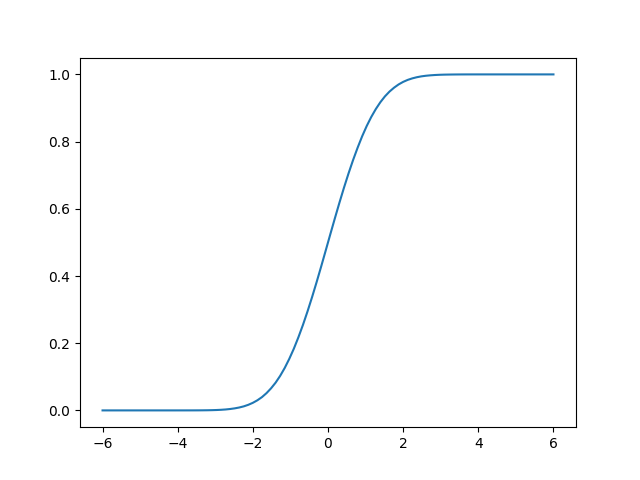
\includegraphics[width=\textheight]{figs/cdf_gau.png}
    \end{figure}
\end{frame}

\subsection{Question 2.3}
\begin{frame}{2.3 - Graph of PDF of X}
    \begin{figure}[!ht]
        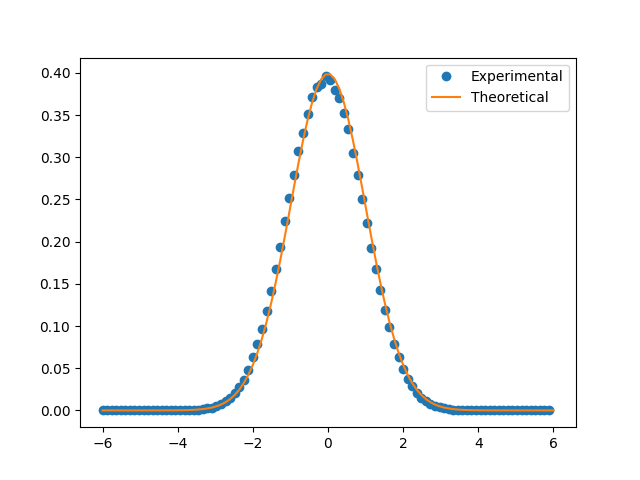
\includegraphics[width=\textheight]{figs/pdf_gau.png}
    \end{figure}
\end{frame}

\subsection{Question 2.4}
\begin{frame}{2.4 - Mean and variance of X}
    The mean and variance are calculated in \texttt{./codes/mean\_var.c}, if \texttt{./codes/gau.dat} is piped into \texttt{stdin}.
\end{frame}

\subsection{Question 2.5}
\begin{frame}{2.5 - Mean and variance of a Gaussian distribution}
    We have
    \begin{equation}
        p_X(x) = \frac{1}{\sqrt{2 \pi}} \exp\left(-\frac{x^2}{2}\right)
    \end{equation}
    The mean is given by
    \begin{align}
        E\left[X\right] &= \int_{-\infty}^{\infty}{x p_X(x) dx} \\
        &= \int_{-\infty}^{\infty}{\frac{x}{\sqrt{2 \pi}} \exp\left(-\frac{x^2}{2}\right) dx}
    \end{align}
    Since this is the integral of an odd function over an odd interval, and the function goes to zero as $x$ diverges,
    \begin{equation}
        E\left[U\right] = 0
    \end{equation}
\end{frame}

\begin{frame}{2.5 (contd)}
    To calculate variance of $X$
    \begin{align}
        \text{var}(X) &= E\left[X - E[X]\right]^2 \\
        &= E\left[X^2\right] \\
        &= \int_{-\infty}^{\infty}{x^2 p_X(x) dx} \\
        &= \int_{-\infty}^{\infty}{\frac{x^2}{\sqrt{2 \pi}} \exp\left(-\frac{x^2}{2}\right) dx} \\
        &= \frac{1}{\sqrt{2 \pi}} \int_{-\infty}^{\infty}{x \cdot x \exp\left(-\frac{x^2}{2}\right) dx}
    \end{align}
\end{frame}

\begin{frame}{2.5 (contd)}
    Integrating by parts, we get
    \begin{align}
        \text{var}(X) &= \frac{1}{\sqrt{2 \pi}}\left(-x \text{exp}\left(\frac{-x^2}{2}\right) + \int{\text{exp}\left(\frac{-x^2}{2}\right) dx}\right) \Bigg|_{-\infty}^{\infty} \\
        &= \frac{1}{\sqrt{2 \pi}} \int_{-\infty}^{\infty}{\text{exp}\left(\frac{-x^2}{2}\right) dx} \\
    \end{align}
    Substituting the Gaussian integral,
    \begin{equation}
        \text{var}(X) = 1
    \end{equation}
\end{frame}

\section{Question 3}
\subsection{Question 3.1}
\begin{frame}{3.1 - Graph of CDF of V}
    \begin{figure}[!ht]
        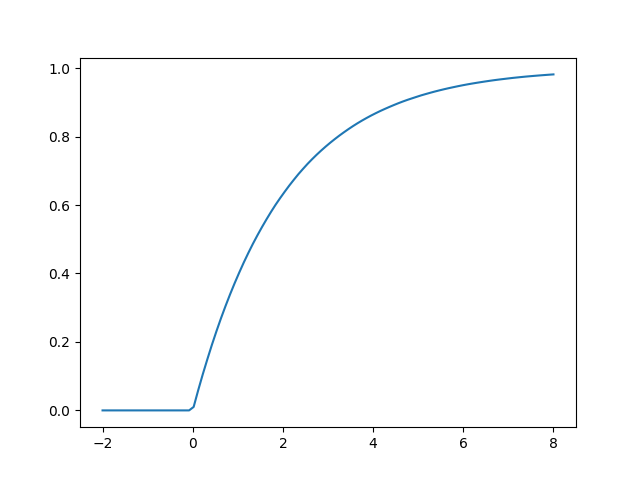
\includegraphics[width=\textheight]{figs/cdf_v.png}
    \end{figure}
\end{frame}

\subsection{Question 3.2}
\begin{frame}{3.2 - CDF of V}
    \begin{align}
        F_V(x) &= \pr{x \leq V} \\
        &= \pr{x \leq -2 \log (1 - U)} \\
        &= \pr{\log (1 - U) \leq \frac{-x}{2}} \\
        &= \pr{1 - U \leq \exp \left(\frac{-x}{2}\right)} \\
        &= \pr{1 - \exp \left(\frac{-x}{2}\right) \leq U} \\
        &= F_U \left(1 - \exp \left(\frac{-x}{2}\right)\right)
    \end{align}
\end{frame}

\begin{frame}{3.2 - (contd)}
    We know $F_U(x)$ from eq \eqref{eq:fu}, so we have
    \begin{align}
        F_V(x) &= F_U \left(1 - \exp \left(\frac{-x}{2}\right)\right) \\
        &= \begin{cases}
            0 & 1 - \exp \left(\frac{-x}{2}\right) < 0 \\
            1 - \exp \left(\frac{-x}{2}\right) & 0 < 1 - \exp \left(\frac{-x}{2}\right) < 1 \\
            1 & 1 - \exp \left(\frac{-x}{2}\right) > 1
        \end{cases}
    \end{align}
    Simplifying, we get
    \begin{equation}
        F_V(x) = \begin{cases}
            0 & x < 0 \\
            1 - \exp \left(\frac{-x}{2}\right) & x \geq 0
        \end{cases}
    \end{equation}
\end{frame}

\end{document}
